\documentclass{article}
\usepackage{iclr2027_conference,times}

% Optional math commands from https://github.com/goodfeli/dlbook_notation.
\input{math_commands.tex}
\usepackage{amsmath,amssymb,mathtools}
\usepackage{booktabs}
\usepackage{graphicx}
\usepackage{xcolor}
\usepackage{microtype}
\usepackage{url}
\usepackage{hyperref}

\newcommand{\method}{\textsc{AdaTransolver}}
\newcommand{\rauec}{\mathrm{rAUEC}}
\newcommand{\todo}[1]{\textit{[Author input needed: #1]}}
\newcommand{\R}{\mathbb{R}}

\title{AdaTransolver: Measure-Aware Spatial Test-Time Scaling for Neural Operators}

% Keep authors anonymous for review. Fill the author block only after the
% collaboration has approved the final author list and affiliations.
\author{Anonymous Authors}

% \iclrfinalcopy
\begin{document}
\maketitle

\begin{abstract}
Neural operators can accept irregular point sets, but this flexibility does not guarantee that a frozen model represents the same continuous operator after the sampling density changes. Local densification changes the empirical measure used by point aggregation and can therefore make additional test-time samples
harmful. We formulate spatial resolution as a test-time compute resource and
introduce \method, a framework that combines variable-point-count training,
measure-aware Physics-Attention, and adaptive spatial allocation. The model is
trained on uniformly sampled subsets with varying cardinality, while a
self-normalized importance correction is applied only to the point-to-slice
reductions at inference. A coarse prediction, a geometry prior, or a lightweight
acquisition head then allocates a fixed point budget across spatial patches.
Across five standard PDE benchmarks, coarse-field allocation lowers the
normalized area under the error--budget curve from the uniform reference of
$1.0$ to $0.574$--$0.937$. On the NACA airfoil benchmark, it reduces relative
$L_2$ error from $0.0169/0.0133/0.0093$ to
$0.0100/0.0070/0.0062$ at $37.5/50/75\%$ point budgets, respectively. A
soft allocation variant obtains $\rauec=0.705$ on an 8.5-million-cell
DrivAerML surface-pressure task. These results show that spatial test-time
scaling is useful when the refinement signal identifies reducible local error
and the frozen operator remains stable under the induced measure shift.
\end{abstract}

\section{Introduction}

Neural operators learn maps between function spaces and can amortize expensive
numerical simulation across many physical configurations
\citep{li2021fno,li2023gino,wu2024transolver}. Their practical appeal is
especially strong for computational fluid dynamics and solid mechanics, where
high-fidelity meshes contain far more points than can be processed during every
training or inference step. Recent architectures address this scale by
compressing irregular meshes into latent tokens, distributing the computation,
or decoupling global state estimation from pointwise decoding
\citep{alkin2024upt,luo2025transolverpp,zhou2026transolver3}. These approaches
make variable input sizes computationally feasible, but they leave a separate
question open: given a fixed inference budget, where should the available
spatial samples be spent?

Uniform subsampling is a robust default, yet it ignores the strongly localized
structure of many PDE solutions. Shocks, boundary layers, contact interfaces,
and stress concentrations occupy only a fraction of the domain. A natural
strategy is therefore to run a coarse prediction and move the remaining point
budget toward regions with large predicted variation. This operation is not a
free composition of an adaptive sampler and an irregular-grid network. Standard
point aggregation uses equal-weight sums or normalized averages. Densifying one
region consequently gives it more empirical mass, even if the underlying
physical area or volume is unchanged. A model may accept the resulting point
set while no longer approximating the same continuous map.

This distinction separates three capabilities that are often conflated:
\emph{irregular-grid compatibility}, which concerns whether a network accepts
different meshes; \emph{measure consistency}, which concerns whether reductions
approximate the same physical integral under different sampling densities; and
\emph{test-time adaptive allocation}, which concerns whether extra spatial
compute is directed to useful regions. Prior work has made substantial progress
on each component separately
\citep{liu2023nuno,berner2026functionspaces,doherty2024quadconv,gao2025discretization,
rowbottom2024gadaptivity}, but their combination remains underexplored.

We study this intersection through \method. The framework first trains a single
Transolver backbone on uniformly sampled subsets whose cardinality varies from
iteration to iteration. At inference, it corrects every point-to-slice reduction
with a relative cell-mass weight, preventing locally dense regions from being
counted repeatedly. A refinement policy then performs a coarse pass, scores
local field variation, aggregates the scores into approximately equal-measure
patches, and redistributes the remaining budget under an explicit density-ratio
constraint. The refined pass uses the same frozen network parameters. Geometry
priors and a lightweight learned acquisition head instantiate the same policy
interface, allowing the source and cost of the refinement signal to be studied
independently from measure correction.

Our contributions are as follows.
\begin{itemize}
    \item We formulate \emph{spatial test-time scaling} for neural operators and
    identify sampling-measure mismatch as the obstacle that prevents irregular
    input support from directly enabling local refinement.
    \item We introduce a measure-aware Physics-Attention rule that inserts
    self-normalized importance weights only into point-to-slice aggregation.
    It reduces to the original model for uniform weights and requires no change
    to slice attention, deslicing, or pointwise layers.
    \item We combine variable-cardinality training with policy-decoupled
    refinement based on coarse-field gradients, geometry priors, or a learned
    acquisition head. Patch-level allocation, a density cap, and farthest-point
    placement maintain global coverage.
    \item We evaluate the resulting accuracy--budget frontier on five standard
    PDE benchmarks and an industrial automotive surface task. We also report
    negative cases that expose when error is unpredictable, irreducible by
    sampling, or too spatially diffuse for local refinement.
\end{itemize}


\begin{figure*}[t]
\centering

\includegraphics[width=\textwidth]{v1/figures/Overview.jpg}
\small
\setlength{\fboxsep}{6pt}
\fbox{\begin{minipage}{0.96\textwidth}
\centering
\textbf{Variable-$N$ training}
$\rightarrow$
\textbf{frozen measure-aware operator}
$\rightarrow$
\textbf{coarse subset $S_0$}
$\rightarrow$
\textbf{field/geometry/head score}
$\rightarrow$
\textbf{patch allocation + FPS}
$\rightarrow$
\textbf{refined subset $S_1$ and reconstruction}
\end{minipage}}
\caption{Overview of \method. Uniform random subsets with variable cardinality
make one checkpoint usable across point budgets. At test time, a refinement
policy reallocates the remaining spatial budget, while measure-aware
point-to-slice aggregation keeps the target physical measure fixed. The model
parameters remain frozen throughout both inference passes.}
\label{fig:overview}
\end{figure*}

\section{Related Work}

\paragraph{Neural operators on irregular geometries.}
Fourier neural operators learn mesh-independent spectral kernels on regular
grids, and Geo-FNO extends this idea to general geometries through learned
deformations \citep{li2021fno,li2023geofno}. GINO couples graph-based integral
operators with a latent grid, while NUNO partitions non-uniform observations to
control interpolation error \citep{li2023gino,liu2023nuno}. Transformer-based
operators such as GNOT, UPT, GAOT, and the Transolver family compress large point
sets into latent tokens before global interaction
\citep{hao2023gnot,alkin2024upt,wen2025gaot,wu2024transolver}. Transolver++ and
Transolver-3 further scale this pattern to million- and hundred-million-cell
geometries \citep{luo2025transolverpp,zhou2026transolver3}. These methods
establish compatibility with irregular inputs and changing resolution. Our
focus is narrower but complementary: whether actively changing the \emph{local}
sampling density preserves the continuous operator and improves a frozen
checkpoint under a finite budget.

\paragraph{Discretization-consistent operator learning.}
Extending finite neural architectures to function spaces requires their
reductions to converge to continuous integrals as the discretization changes
\citep{berner2026functionspaces}. Monte Carlo convolution corrects non-uniform
point-cloud sampling with inverse-density weights
\citep{hermosilla2018montecarlo}, while QuadConv evaluates learned continuous
kernels through numerical quadrature on irregular PDE data
\citep{doherty2024quadconv}. Discretization mismatch can remain substantial even
for architectures whose parameters do not depend on grid resolution
\citep{gao2025discretization}. Related work also studies discretization-invariant
maps between neural fields and quadrature-aware normalization
\citep{wang2022din,kim2026quadnorm}. We apply the same functional principle to
Physics-Attention, but use it to enable an active test-time intervention: the
sampling density is intentionally changed to improve the accuracy--compute
frontier.

\paragraph{Adaptive meshes and test-time refinement.}
Classical adaptive discretization reduces numerical error by refining elements
whose residual or estimated contribution is large. Learned variants predict
mesh density or node relocation for numerical solvers
\citep{huang2021meshgeneration,obiols2023adarnet,rowbottom2024gadaptivity}.
MeshGraphNets similarly operates on mesh graphs and supports remeshing in
learned simulation \citep{pfaff2021meshgraphnets}. These methods primarily use
adaptivity to construct a mesh for a numerical or recurrent simulator. In
neural-operator test-time scaling, PDE-Refiner adds iterative denoising steps and
operator splitting adds test-time operator composition
\citep{lippe2023pderefiner,serrano2026splitting}. \method instead scales the
spatial sample budget of one frozen feed-forward operator. This axis is
orthogonal to increasing model size, pretraining data, or the number of
refinement iterations.

\section{Method}

\subsection{Problem formulation}

Let $\Omega$ be a physical domain with target measure $\mu$, and let
$\mathcal{G}_\theta$ map an input function $f$ to a solution field $u$.
For each test instance, a high-resolution candidate discretization
$\mathcal{X}_H=\{x_i\}_{i=1}^{N_H}$ is available, but the operator may be
evaluated on at most $N_f<N_H$ points. The goal is to select a subset
$S\subset\{1,\ldots,N_H\}$, evaluate the frozen model on $\mathcal{X}_S$, and
reconstruct the full field with lower error than uniform sampling at the same
final point count. The end-to-end computation includes selection, operator
evaluation, and reconstruction; we separately report point-budget results and
identify equal-time evaluation as an outstanding requirement.

\subsection{Variable-cardinality training}

A checkpoint trained only at one point count can fail before any allocation
policy is considered. We therefore treat every benchmark as an unstructured
point cloud during training. At iteration $t$, we draw
\begin{equation}
N_t \sim \mathcal{U}\!\left(\lceil\rho_{\min}N_H\rceil,N_H\right),
\qquad
S_t \sim \operatorname{UniformSubset}(N_H,N_t),
\end{equation}
and compute the task loss only on $S_t$. Standard two-dimensional benchmarks
use $\rho_{\min}=0.3$; very large three-dimensional meshes use a smaller range
such as $1$--$10\%$. The subset is shared across examples in a minibatch and,
for temporal tasks, across the rollout. This training rule changes the number
of observations without introducing a non-uniform spatial density. It should
therefore be distinguished from density-adaptive training, which did not
improve the strongest NACA checkpoint in our experiments.

\subsection{Measure-aware Physics-Attention}

Transolver assigns each point feature $h_i$ to $G$ physical slices using
non-negative soft assignments $a_{ig}$, normalized over slices for each point.
The standard slice token is
\begin{equation}
z_g = \frac{\sum_{i\in S} a_{ig}v(h_i)}
           {\sum_{i\in S} a_{ig}}.
\label{eq:vanilla-token}
\end{equation}
Under uniform sampling, Eq.~\eqref{eq:vanilla-token} is a self-normalized Monte
Carlo estimate of an integral over $\mu$. If points are instead sampled from a
density $q$, the same expression integrates against $q\,d\mu$ and overweights
locally dense regions.

Let $m_i$ denote the physical mass represented by selected point $i$. On meshes
with cell areas or volumes, $m_i$ is obtained directly; otherwise we estimate it
by assigning every candidate point to its nearest selected point. With
$\bar m=|S|^{-1}\sum_{i\in S}m_i$, we define
\begin{equation}
c_i(\beta)=\left(\frac{m_i}{\bar m}\right)^\beta,
\qquad 0\leq\beta\leq1,
\end{equation}
and replace Eq.~\eqref{eq:vanilla-token} by
\begin{equation}
z_g^{(\beta)} =
\frac{\sum_{i\in S} c_i(\beta)a_{ig}v(h_i)}
     {\sum_{i\in S} c_i(\beta)a_{ig}}.
\label{eq:measure-token}
\end{equation}
Here $\beta=0$ recovers the original point-count aggregation, $\beta=1$ is the
full measure correction, and intermediate values trade finite-sample bias
against variance. We select $\beta$ on a validation set, typically obtaining
$0.5$--$0.75$.

The correction is deliberately local to the two sums in
Eq.~\eqref{eq:measure-token}. Slice assignment remains normalized over slices,
self-attention acts only on the $G$ tokens, deslicing remains pointwise, and
feature normalization acts over channels. Consequently, setting $c_i=1$ exactly
recovers the original computation. In a replication audit, full correction
reduced the deviation caused by local point replication from $2.0\times10^{-2}$
to $4.7\times10^{-7}$.

\paragraph{Consistency.}
Suppose $x_i$ are sampled independently from $q$ and
$c_i\propto d\mu/dq(x_i)$. If the denominator is nonzero and the token features
are integrable, the strong law of large numbers applied to the numerator and
denominator gives
\begin{equation}
z_g^{(1)} \xrightarrow[]{a.s.}
\frac{\int_\Omega a_g(x)v(h(x))\,d\mu(x)}
     {\int_\Omega a_g(x)\,d\mu(x)}.
\end{equation}
Thus full correction converges to a token defined by the target physical
measure rather than by the chosen sampling density. This argument does not
guarantee finite-sample improvement; it only removes one source of systematic
measure shift.

\subsection{Adaptive spatial allocation}

Our primary policy uses one coarse pass and one refined pass.

\paragraph{Coarse prediction and local score.}
We draw a uniform initial subset $S_0$ with $N_0=\rho_0N_H$ points, using
$\rho_0=0.25$ on the standard benchmarks. From the normalized coarse prediction
$\widehat u^0$, we estimate local field variation with $k$ nearest neighbors:
\begin{equation}
r_i = \frac{1}{k}\sum_{j\in\mathcal{N}_k(i)}
\frac{\|\widehat u_i^0-\widehat u_j^0\|_2^2}
     {\|x_i-x_j\|_2^2+\epsilon}.
\label{eq:grad-score}
\end{equation}
The score uses no test labels. For automotive surfaces, a soft Laplacian score
is more stable than hard selection and is discussed in
Section~\ref{sec:drivaer}.

\paragraph{Patch allocation.}
We partition the candidate discretization into $K$ approximately equal-measure
patches with spatial clustering. For patch $P_k$, let $A_k$ be its physical
mass and let $R_k$ be the mean score among coarse points in the patch. We rank
patches by estimated gain per available point,
\begin{equation}
\eta_k = \frac{A_kR_k}{|P_k\setminus S_0|+\epsilon},
\end{equation}
and greedily allocate the remaining $N_f-N_0$ points. To preserve global
coverage, the final patch densities $d_k=|S_1\cap P_k|/A_k$ satisfy
\begin{equation}
\frac{\max_k d_k}{\min_k d_k+\epsilon}\leq\kappa.
\end{equation}
Within each selected patch, farthest-point sampling places new points relative
to the existing subset. This separates \emph{which region} receives compute
from \emph{how points cover that region}.

\paragraph{Policy variants.}
A geometry-prior policy uses an exponential function of distance to a known
boundary and skips the coarse pass. A learned policy attaches a lightweight
Transolver acquisition head to first-block features and predicts a local
gradient target. The latter uses only approximately one eighth of the backbone
depth and is $2$--$4.5\times$ cheaper than a full coarse forward in the current
implementations. All variants share the same measure-aware refined pass.

\subsection{Evaluation metrics}

For a reconstructed field $\widetilde u$ on the full candidate mesh, we report
the mass-weighted relative error
\begin{equation}
E(S)=\left(
\frac{\sum_{i=1}^{N_H} a_i\|\widetilde u_i-u_i\|_2^2}
     {\sum_{i=1}^{N_H} a_i\|u_i\|_2^2+\epsilon}
\right)^{1/2},
\end{equation}
where $a_i$ is physical cell mass when available. To summarize an
accuracy--budget curve, we use
\begin{equation}
\rauec =
\frac{\int_{\mathcal{B}} E_{\mathrm{method}}(b)\,db}
     {\int_{\mathcal{B}} E_{\mathrm{uniform}}(b)\,db},
\qquad \mathcal{B}=\{0.375,0.50,0.75\}.
\end{equation}
Values below one improve on equal-final-point uniform sampling. This metric does
not by itself establish equal-time efficiency because adaptive policies may
perform an additional coarse pass.

\section{Experiments}

\subsection{Setup}

We use the standard Transolver PDE collection: Darcy flow, elasticity, pipe
flow, NACA airfoil flow, and plasticity. The tasks cover regular grids,
unstructured point clouds, localized interfaces, shocks, and contact regions.
The backbone is trained with variable point counts and then frozen. The main
comparison holds the final point set, reconstruction method, test examples, and
random seeds fixed across acquisition policies. Uniform sampling is normalized
to $\rauec=1$. We compare geometry-prior allocation, the coarse-field score in
Eq.~\eqref{eq:grad-score}, farthest-point coverage, and the learned acquisition
head where available. Hyperparameters $\beta$ and $\kappa$ are selected on a
validation split.

For industrial scale, we evaluate surface-pressure prediction on DrivAerML.
Each vehicle has approximately $8.5$ million surface cells. The input contains
normalized positions and surface normals, and the output is standardized
pressure. Current results use 50 test vehicles and a one-million-point candidate
pool for allocation. \todo{Verify the final train/validation/test split, random
seeds, and exact pool construction against the release scripts.}

\subsection{Accuracy--budget scaling across PDE benchmarks}

Table~\ref{tab:main-results} reports the main point-budget results. Coarse-field
allocation improves on uniform sampling on all five benchmarks, with the
largest reduction on NACA airfoil ($\rauec=0.574$) and the smallest on Darcy
flow ($0.937$). The ordering is physically plausible: airfoil shocks,
elasticity stress concentrations, and plastic contact regions are localized,
whereas the dominant Darcy error is more spatially diffuse. The learned head
matches the full coarse policy on airfoil and remains competitive on pipe,
elasticity, and plasticity while reducing acquisition cost. Geometry priors are
useful but consistently weaker than the data-dependent coarse score in this
evaluation.

\begin{table}[t]
\caption{Equal-final-point accuracy--budget results. Lower $\rauec$ is better;
uniform sampling is $1.000$. Full-grid relative $L_2$ reports the validation
quality of the variable-$N$ checkpoint. Dashes denote unavailable learned-head
results. Values should be re-exported from the final experiment registry before
submission.}
\label{tab:main-results}
\centering
\small
\begin{tabular}{lrrrr}
\toprule
Benchmark & Full-grid $L_2$ & Geometry & Coarse field & Learned head \\
\midrule
Airfoil    & 0.0063 & 0.788 & \textbf{0.574} & 0.575 \\
Pipe       & 0.0048 & 0.870 & \textbf{0.811} & 0.819 \\
Elasticity & 0.0100 & 0.893 & \textbf{0.707} & 0.775 \\
Plasticity & 0.0030 & 0.871 & \textbf{0.769} & 0.783 \\
Darcy      & 0.0136 & 0.988 & \textbf{0.937} & -- \\
\bottomrule
\end{tabular}
\end{table}

\begin{figure*}[t]
\centering
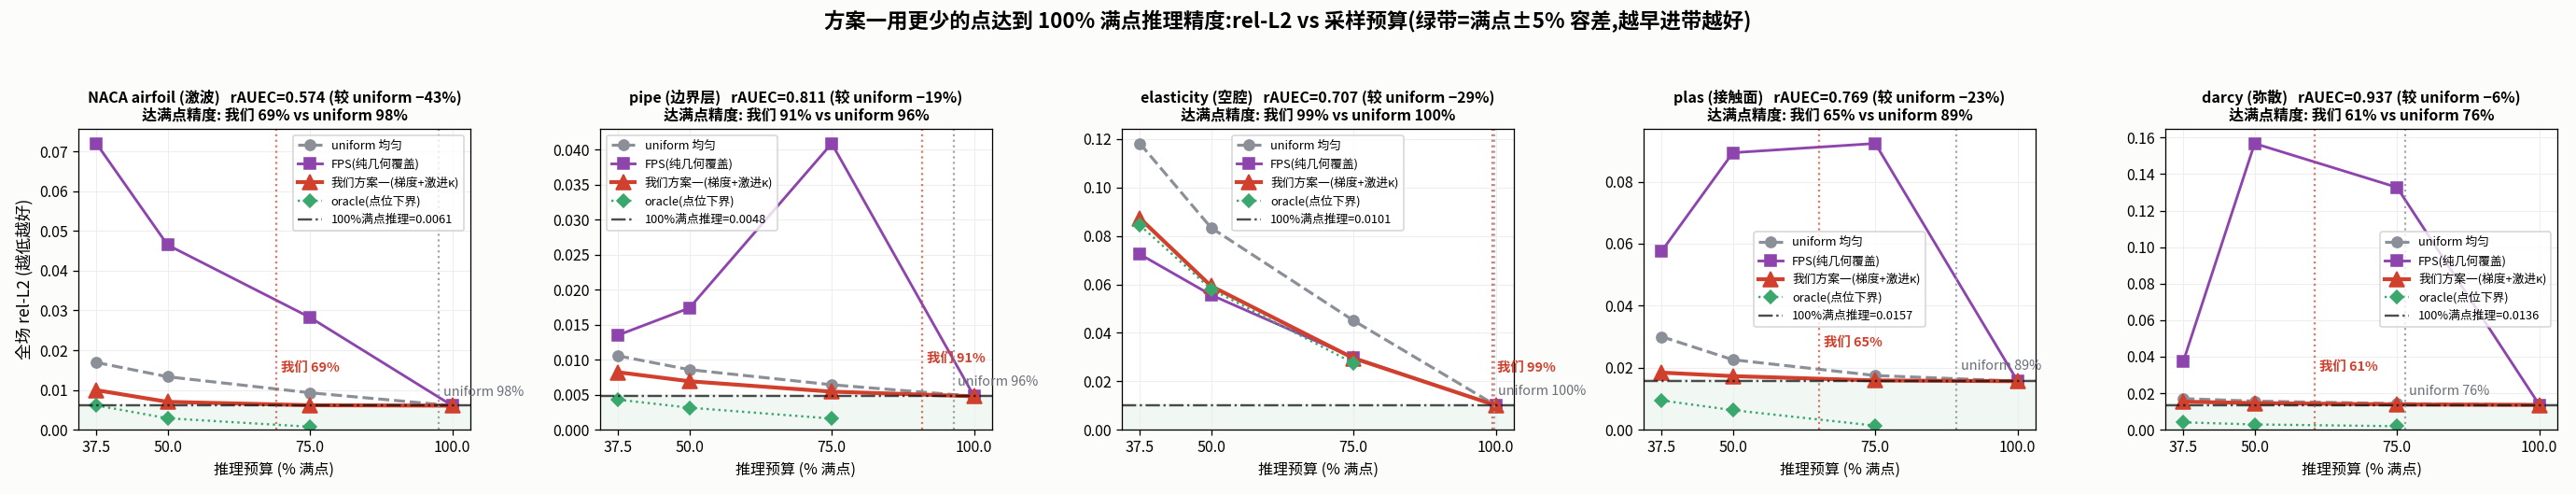
\includegraphics[width=\textwidth]{figures/multibench_curves.png}
\caption{Error--budget curves for coarse-field adaptive allocation on five PDE
benchmarks. The adaptive policy reaches the full-grid checkpoint error with
approximately $69\%$, $91\%$, $99\%$, $65\%$, and $61\%$ of the candidate points
on airfoil, pipe, elasticity, plasticity, and Darcy, respectively. The embedded
labels are retained from the experiment artifact and will be re-exported in
English for submission.}
\label{fig:multibench}
\end{figure*}

\subsection{NACA airfoil analysis}

The airfoil task provides the clearest spatial scaling curve. At point budgets
of $37.5\%$, $50\%$, and $75\%$, uniform sampling obtains relative errors
$0.0169$, $0.0133$, and $0.0093$, respectively. Coarse-gradient allocation with
$\kappa=16$ obtains $0.0100$, $0.0070$, and $0.0062$. The last value matches the
full-grid checkpoint error of $0.0061$ within rounding while using one quarter
fewer final points. Across five visualized test examples at a $50\%$ budget,
relative error falls by $46$--$69\%$ because the refined samples concentrate on
the moving shock and near-surface region (Figure~\ref{fig:naca-qual}).

The density cap controls whether the policy is sufficiently decisive. Raising
$\kappa$ from $4$ to $16$ lowers $\rauec$ from $0.813$ to $0.574$, after which
performance saturates. A coverage-only farthest-point baseline is much worse on
four of five benchmarks, showing that the gain does not arise merely from a
more regular point set. Density-adaptive \emph{training} also fails to improve
the strongest NACA checkpoint. The successful combination is instead uniform
variable-$N$ training, aggressive test-time allocation, and measure correction.

\begin{figure*}[t]
\centering
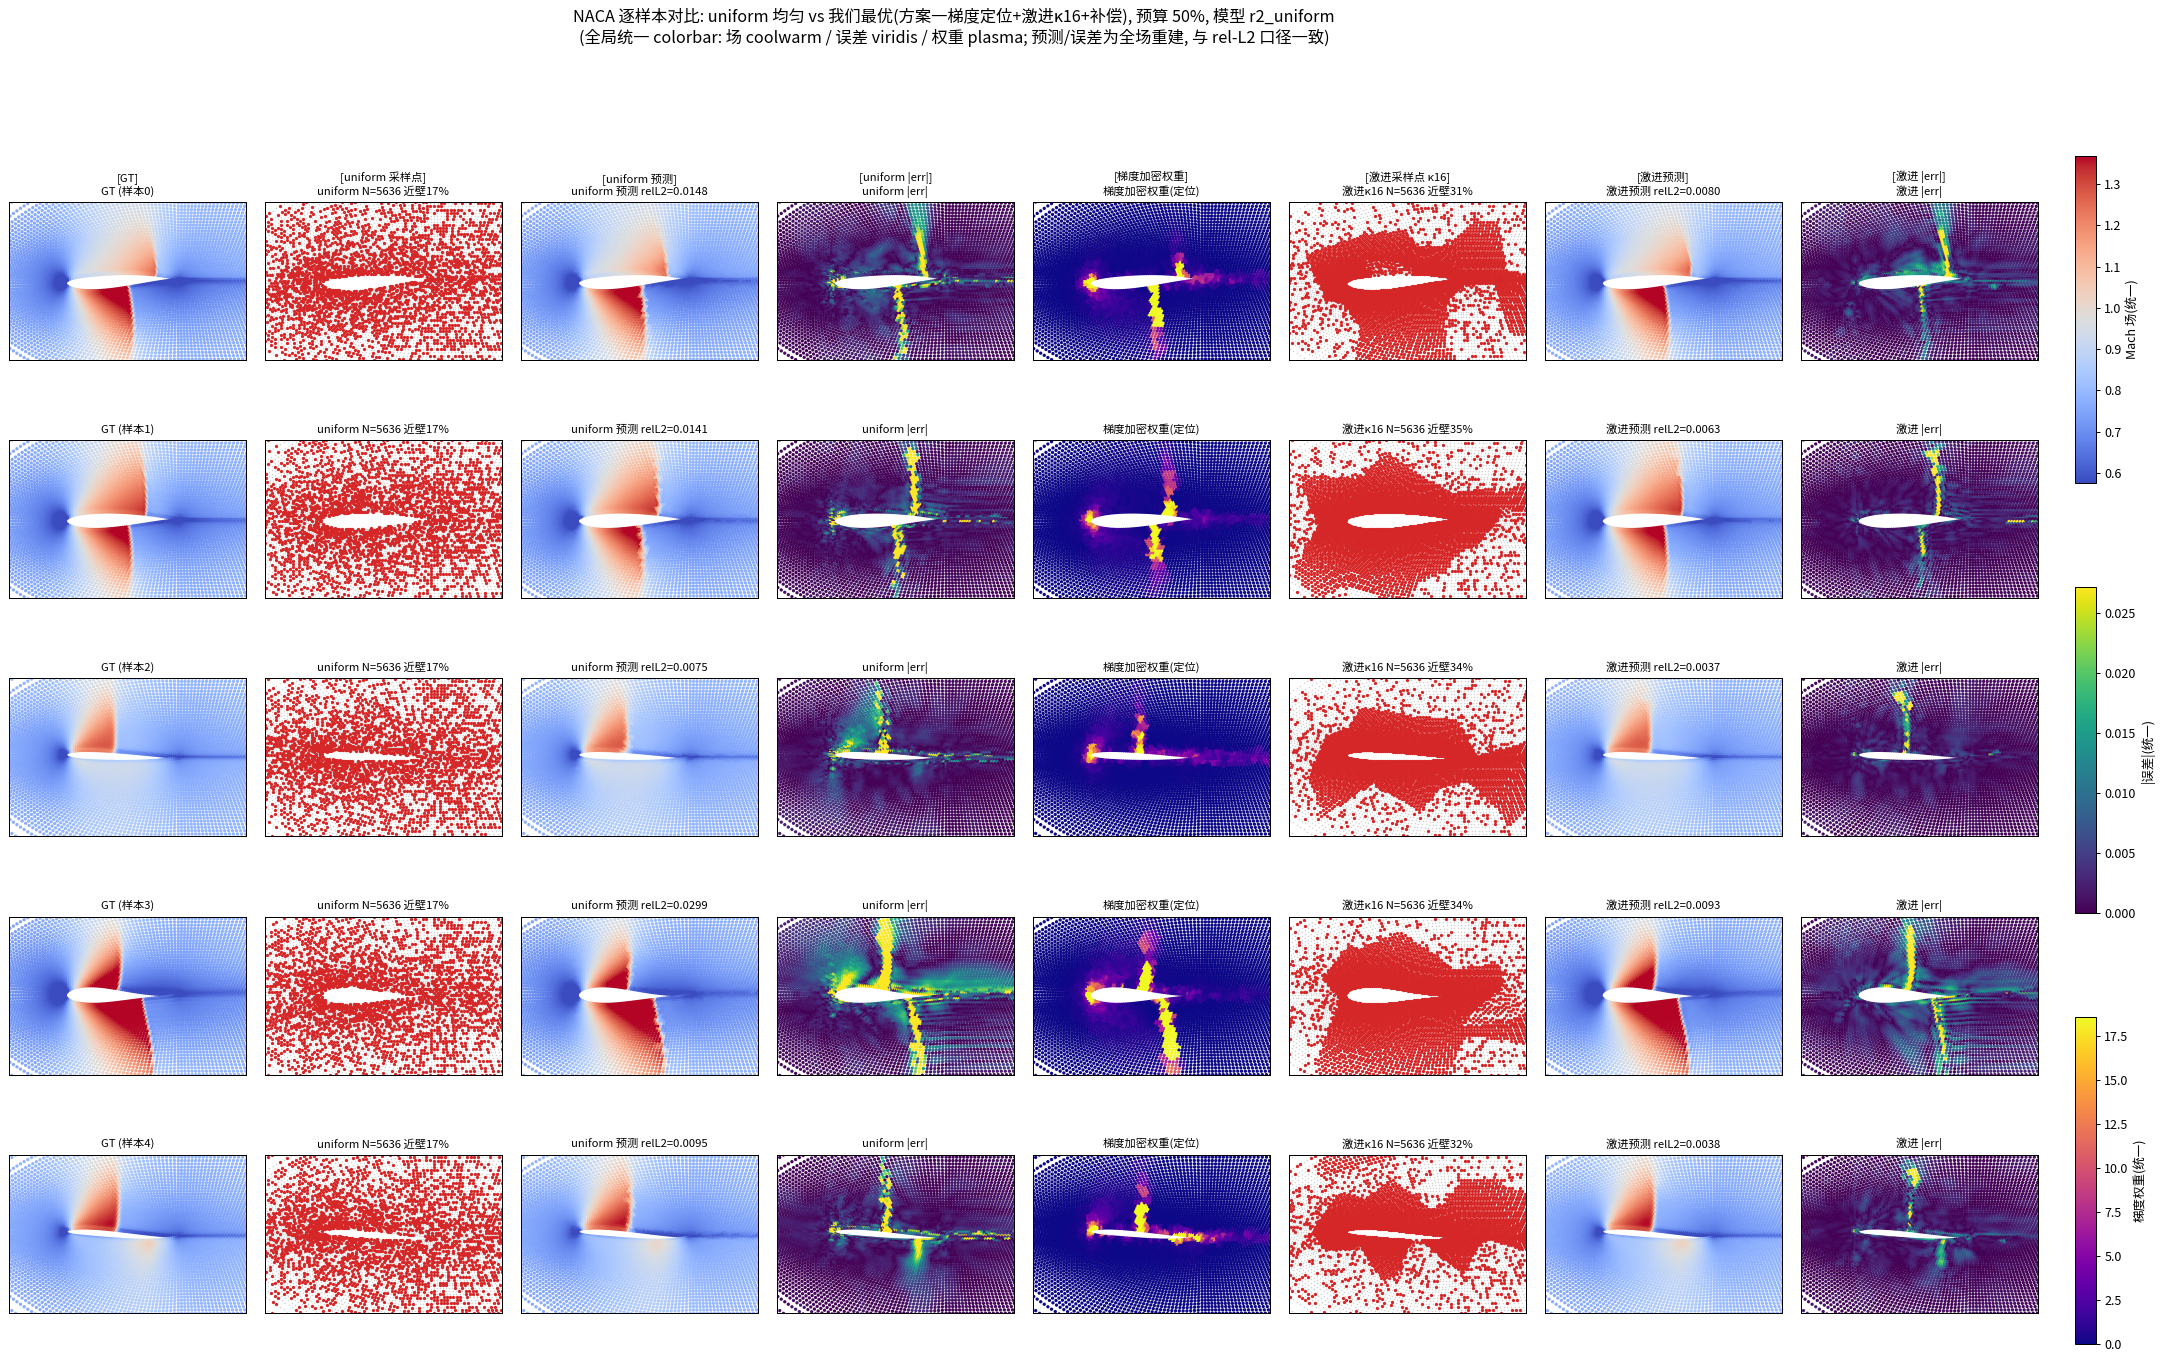
\includegraphics[width=\textwidth]{figures/naca_qualitative.png}
\caption{NACA qualitative comparison at a $50\%$ final point budget. Columns
show the reference field, uniform samples and prediction, uniform error,
coarse-gradient acquisition score, adaptive samples and prediction, and
adaptive error. Adaptive samples track the shock location across examples. The
embedded labels are retained from the experiment artifact and will be
re-exported in English for submission.}
\label{fig:naca-qual}
\end{figure*}

\subsection{Industrial automotive surfaces}
\label{sec:drivaer}

Hard patch selection initially failed on DrivAerML even though an oracle
reconstruction diagnostic showed that the selected locations were useful. On
the same adaptive point set, oracle reconstruction error decreased from $0.153$
to $0.129$, but model error increased sharply. This isolates a layout shift in
the frozen uniformly trained checkpoint rather than a failure of the sampling
indicator. Replacing hard selection with a soft Laplacian weighting and using
partial correction ($\beta=0.5$) yields $\rauec=0.705$ for surface pressure. At
$37.5\%$, $50\%$, and $75\%$ budgets, relative error decreases by approximately
$34\%$, $32\%$, and $20\%$ against uniform sampling
(Figure~\ref{fig:drivaer}). This case illustrates why compatibility, measure
consistency, and allocation should be audited separately.

\begin{figure}[t]
\centering
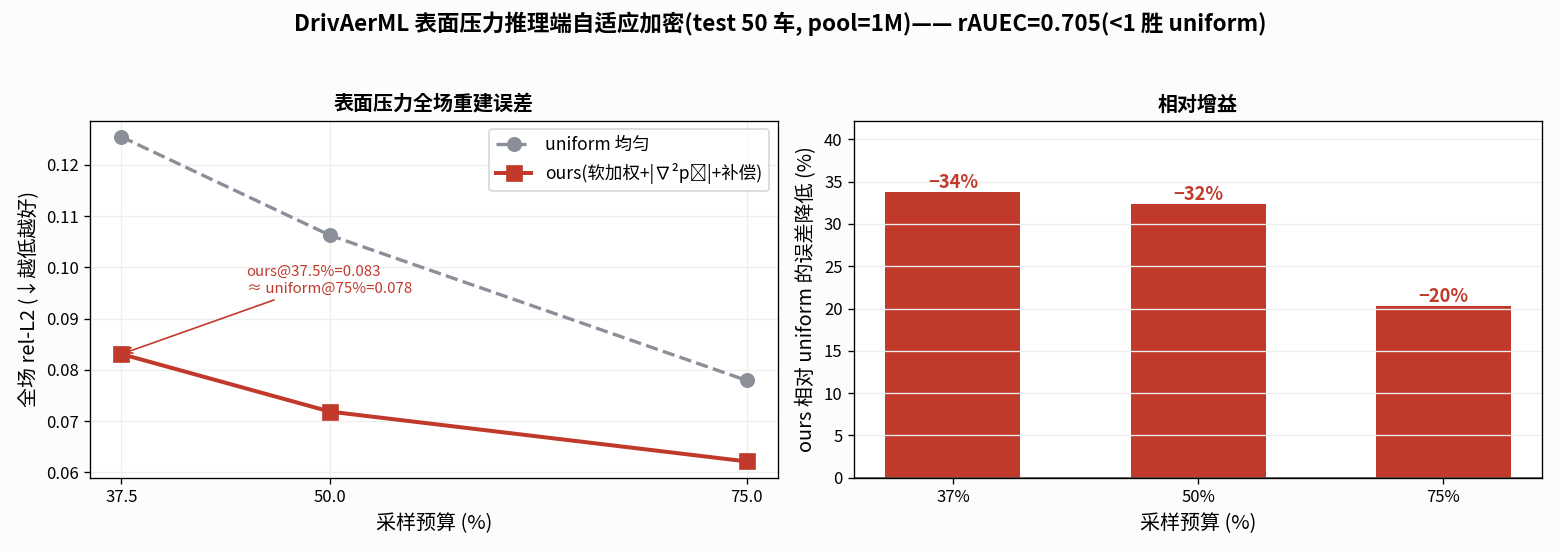
\includegraphics[width=\columnwidth]{figures/drivaer_curve.png}
\caption{DrivAerML surface-pressure error under soft Laplacian allocation. The
method improves all three evaluated point budgets and yields
$\rauec=0.705$. The embedded labels are retained from the experiment artifact
and will be re-exported in English for submission.}
\label{fig:drivaer}
\end{figure}

\subsection{Failure modes and diagnostic evidence}

An auxiliary 21k-parameter error predictor clarifies when spatial scaling should
not be expected to help. Learned error allocation is effective on airfoil
($\rauec=0.763$) and elasticity ($0.927$), approximately neutral on
Navier--Stokes and plasticity, and slightly worse than uniform on pipe and Darcy
($1.025$ and $1.038$). The failures have different causes. Navier--Stokes error
is difficult to predict after chaotic rollout; plasticity has many output
channels whose error regions do not coincide; pipe boundary-layer gains occupy
too little of the global metric; and Darcy error is predictable but dominated
by model bias that additional samples do not remove.

These observations suggest a three-factor diagnostic: adaptive sampling helps
when local error is predictable from permitted test-time information, reducible
by additional spatial observations, and concentrated enough to affect the
global objective. Measure correction prevents a density shift from corrupting
the operator, but it cannot make an uninformative acquisition score useful or
remove irreducible model bias.

\section{Discussion}

The main result is not that one gradient heuristic solves every PDE. It is that
spatial resolution can become a controllable test-time resource once the
operator and the allocation policy are separated. Variable-cardinality training
addresses the input-count shift, measure-aware aggregation addresses the
sampling-density shift, and the policy decides where marginal resolution is
valuable. This decomposition makes failures interpretable: a point-count audit,
a replication audit, an oracle reconstruction audit, and a score-to-gain audit
test distinct assumptions.

The evidence also exposes a finite-sample tension. Full importance correction
is asymptotically aligned with the target measure, but partial correction often
performs better at the point counts used in practice. We interpret $\beta<1$ as
a bias--variance trade-off, not as exact invariance. Future work should replace
validation-tuned exponents with estimators that account for uncertain cell mass
and token-specific effective sample size. The same principle should be audited
for any spatial reduction added to the backbone, including global pooling or
spatial normalization.

Our current evaluation has four important boundaries. First, the main tables
equalize final point count rather than end-to-end wall-clock time; the extra
coarse pass must be compared with a higher-budget one-pass uniform baseline.
Second, paired confidence intervals and seed-level statistics have not yet been
consolidated across all result files. Third, several figures require an English
re-export and a single frozen evaluation registry. Fourth, the strongest
industrial result uses a task-specific soft Laplacian policy, so broader claims
about a universal hard-refinement rule would be unsupported. These limitations
do not change the observed point-budget improvements, but they bound the current
claim to an accuracy--sampling frontier rather than a complete latency scaling
law.

\section{Conclusion}

We introduced \method, a framework for spatial test-time scaling of neural
operators. Its central design principle is that locally adding points should
change spatial resolution without changing the physical measure represented by
the model. Variable-cardinality training, measure-aware Physics-Attention, and
policy-decoupled refinement together improve equal-point-budget error across
five PDE benchmarks and an industrial automotive surface task. The largest gain
occurs when difficult regions are localized and additional samples reduce their
error; diffuse, unpredictable, or model-bias-dominated errors define the method's
present boundary. Establishing equal-time gains with consolidated uncertainty
estimates is the next requirement for a full test-time compute scaling claim.

\bibliography{references}
\bibliographystyle{iclr2026_conference}

\appendix

\section{Draft Reproducibility Checklist}

\begin{itemize}
    \item \textbf{Backbone:} Transolver or Transolver-3 with unstructured input
    handling; variable point count sampled uniformly without replacement.
    \item \textbf{Coarse policy defaults:} $\rho_0=0.25$, $k=8$ nearest
    neighbors, $K=48$ patches, one refinement round.
    \item \textbf{Point budgets:} $37.5\%$, $50\%$, and $75\%$ of the candidate
    discretization.
    \item \textbf{Correction:} nearest-selected-point cell mass with
    $\beta\in\{0,0.5,0.75,1\}$ selected on validation data.
    \item \textbf{Baselines:} one-pass uniform, two-pass uniform, geometry
    prior, coverage-only FPS, learned acquisition head, and oracle
    reconstruction for diagnosis only.
    \item \textbf{Outstanding before submission:} paired bootstrap confidence
    intervals, end-to-end latency and memory, a final seed registry, and the
    official ICLR 2027 style.
\end{itemize}

\end{document}
